\chapter{序論}
\thispagestyle{fancy}
\nobreak
\section{研究背景と目的}
本研究は「オーディトリウムの“底”で演奏を聴く」という旧態依然とした鑑賞形態並びにそれに基づく決定論的設計法に対し、建築音響学の観点から新たな息吹を吹き込むことで、次世代の建築を設計するための礎を築こうとするものである。

\subsection{1階座席の音響的評価}
1階座席床面には大きな吸音力を持つ聴衆と椅子が集中しており、これはホール空間全体の吸音力のうち大半を占める(500Hzで7割程度)$^{\text{\cite{01-2}{\cite{椅子吸音}}}}$。いわば、私たちは座席吸音体(聴衆+椅子)の中で演奏を聴いている。

\subsection{2階バルコニー最前列席の音響的評価}
ここで、収容人数や舞台へ向けての視野を確保する観点から、オーディトリウムにバルコニー席を設けることが多々ある。このとき、前方に客席がないバルコニー先端部はホール空間へ張り出した特異な場であり、ほぼ宙に浮いた状態である。
\\ さて、2階バルコニー最前列の座席は、音響的に高い評価を得ることが多い$^{\text{\cite{01-1}{\cite{AAAD}}}}$。これは、座席吸音体から相対的に離れた場所に位置するため、エネルギ減衰の少ない有効な直接音や反射音を得やすいことに起因すると定性的には推察されている(\figref{2階バルコニー最前列席の音場})。
\\ また、この“宙に浮いた席”を増やす目的でバルコニーに吹き抜けを設けた「フライングバルコニー」が計画されることもある。詳細は後述する。
\\
\begin{figure}[h]
    \centering
    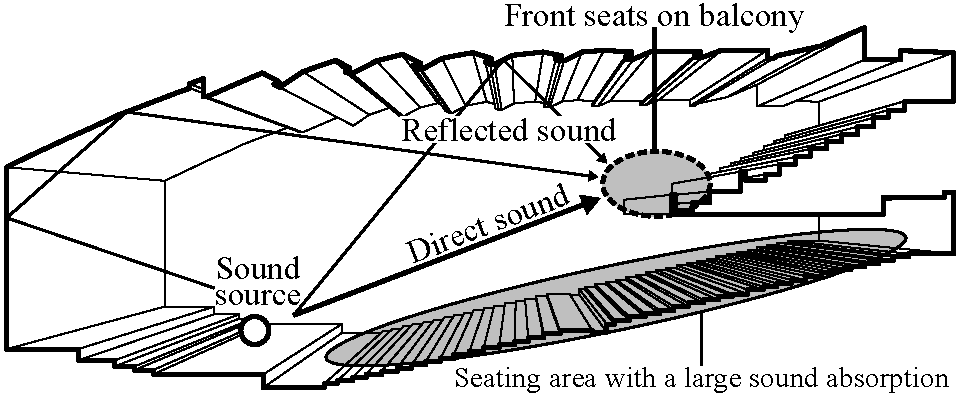
\includegraphics[keepaspectratio,scale=0.8]{01_att/second_balcony.pdf}
    \caption{\hspace{1mm}Sound field at front seats on balcony}
    \label{fig:2階バルコニー最前列席の音場}
\end{figure}

%-------------------------------------------------------------
\newpage
\subsection{評価対象領域の拡張}
一方、建築音響学が体系化した1900年以後$^{\text{\cite{01-3}}}$、ホールの音響性能について種々研究が行われているものの、音場測定や解析シミュレーションによる音場の評価は、当然のことながら、建築的に確定された客席床面(床面上高さ1$\sim$2m)における面的評価$^{\text{\cite{受音点選定}{\cite{最適位置}}}}$に留まっており、ホール空間全体を評価対象とした設計研究は皆無$^1$である。本研究では、前節で述べた知見を踏まえ、評価対象領域を床面遠方音場へと拡張した評価を試みる(\figref{評価対象領域の拡張})。
\\ また、ホール空間で美しい響きを生み出すにあたり、ホールの室容積は人間を収容するには冗長な大きさを要する。規模により異なるものの、室容積から算出されるホールの天井高はおおよそ10$\sim$20mである。ホール空間は人が鑑賞可能なエリアを断面方向含め無数に拡張できるというポテンシャルを秘めているにも関わらず、オーディトリウムの底で鑑賞をするという様式は依然として変わっていない。
\\ 
\begin{figure}[htbp]
    \centering
    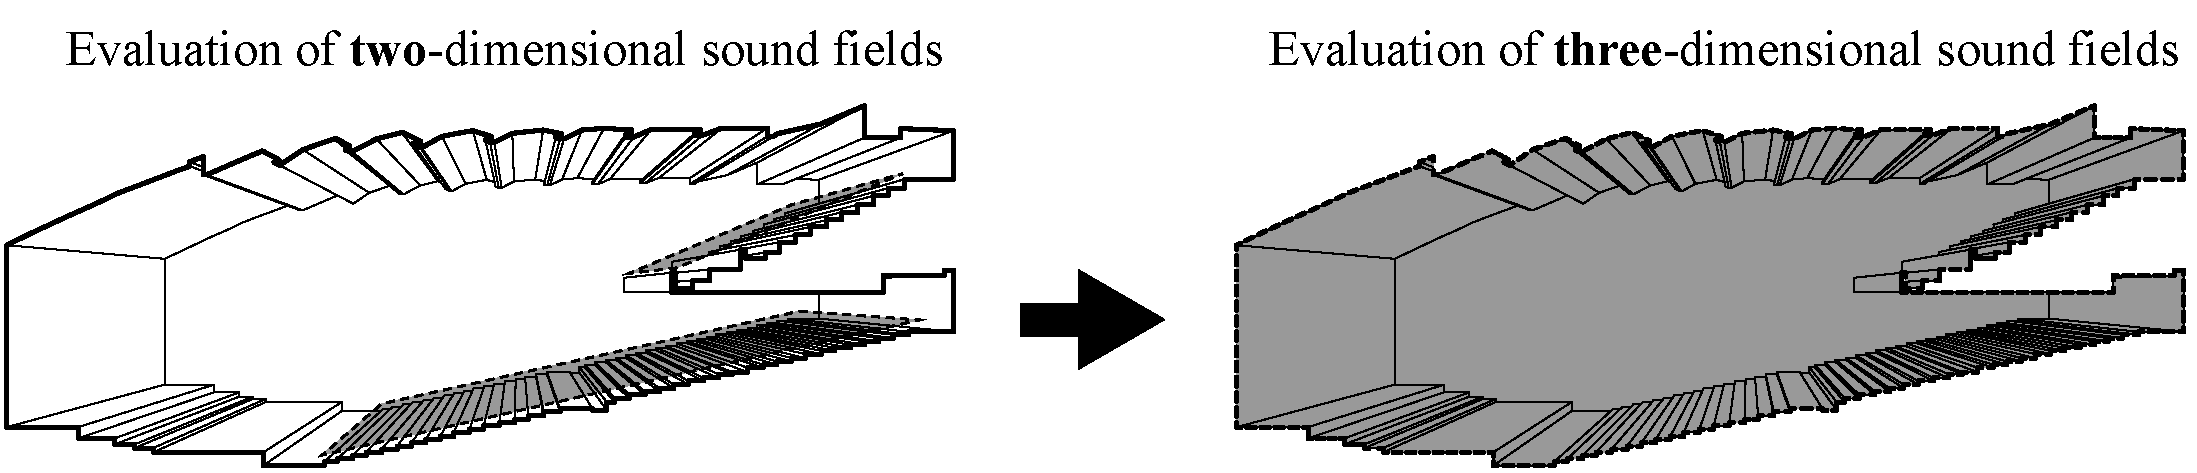
\includegraphics[keepaspectratio,scale=0.41]{01_att/evaluate_area.pdf}
    \caption{\hspace{1mm}\textbf{Expanding of evaluation area}}
    \label{fig:評価対象領域の拡張}
\end{figure}

\addtocounter{footnote}{1}
\footnotetext{観測点を3次元に配置した研究は行われている$^{\text{\cite{綿谷}}}$(壁面に対し床面あるいは天井面が高度な吸音性の場合、3次元拡散音場に用いるSabineの残響式で計算した値よりも残響時間が長くなることから、2次元拡散音場の音響性状を明らかにする研究。なお、コンサートホールも吸音面が偏在した空間ではあるが、壁面に拡散体が多数設置されているため、この音響性状は生じない)。}

\pagebreak
\subsection{研究目的}
本研究は、コンサートホール音場の評価対象領域を、吸音力の大きな座席面近傍音場から3次元的に拡張し、床面遠方音場(\figref{座席面遠方音場})の音響物理特性を拡散性の観点から明らかにすることにより、従来の面的評価並びにそれに基づく決定論的設計法に新たな可能性を見出すことを目的とするものである。
\begin{figure}[htbp]
    \centering
    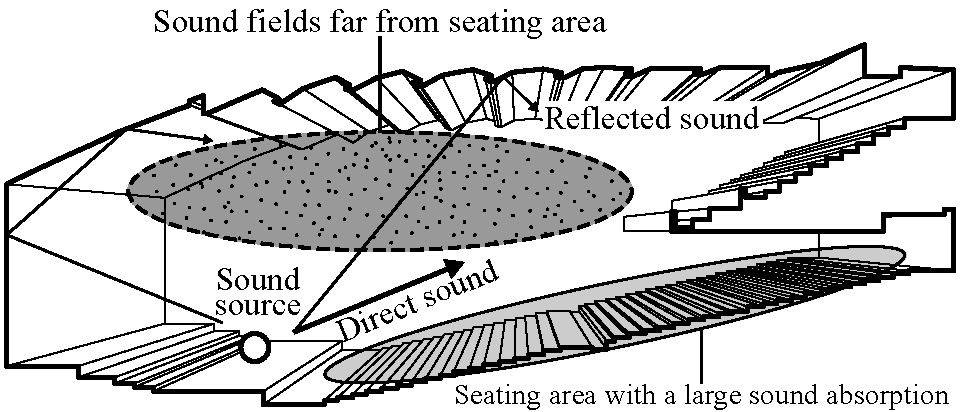
\includegraphics[keepaspectratio,scale=0.8]{01_att/zasekimen_enpo_English.pdf}
    \caption{\hspace{1mm}Sound field far from seating area}
    \label{fig:座席面遠方音場}
\end{figure}

%-------------------------------------------------------------
\newpage
\section{室内音響物理指標について}
ホール空間などにおいて特に重要な4つの要素感覚(音量感、残響感、明瞭性、広がり感)に対応するとして定義された、代表的な室内音響物理指標を以下に述べる$^{\text{\cite{01-3}}{\text{\cite{響きのパラメータ}}}}$。

\subsection{音量感に関する物理指標}
音の大きさは、到来する音の全エネルギー量に対応するとして、\STG が \textbf{式}\ref{eq:STG}より定義されている。これは、直接音を含む全ての反射音エネルギーを、音源のパワーに準ずるエネルギーによって基準化した量である。ここで、$p(t)$は観測点における音圧、$p_{A10}(t)$は無響室内10m点における音圧である。受聴レベルは、音量感だけでなく広がり感や残響感の大小にも影響を与えることが知られており、室内音場の性質を表す基本的かつ重要な物理指標である。

\begin{equation}
  \label{eq:STG}
  G = 10\log_{10}{\frac{\displaystyle\int_0^{\infty}p^2(t)dt}{\displaystyle\int_0^{\infty}p_{A10}^2(t)dt}} \dB
\end{equation}

\subsection{響きの量に関する物理指標}
聴感的な響きの長さは、残響過程の比較的初期の減衰の仕方に影響を受けることが明らかにされており、初期残響時間$EDT$[s]が残響感に対応する物理指標として提案されている。これは、残響時間が60dB減衰に要する時間であるのに対し、初期の10dB減衰の傾きから算出した残響時間であり、10dB減衰に要する時間を6倍にしたものとして算出される。

\subsection{明瞭性に関する物理指標}
初期反射音は、直接音をエネルギー的に補強し聴感的な明瞭性を高める効果がある。そこで、この初期反射音のエネルギーに着目し、音楽の明瞭度に対応する物理指標として初期/ 後期エネルギー比 \Clarity(Clarity) が、話声に対応する物理指標として$D_{50}$(Deutlichkeit)がそれぞれ定義されている。これらは、後期反射音に対する初期反射音エネルギーの割合を表したものである。初期反射音エネルギーが増加するほど値は大きくなり、聴感的な明瞭性が増すことを意味する。
\begin{equation}
    \label{eq:c80}
  C_{80} = 10\log_{10}{\frac{\displaystyle\int_0^{80}p^2(t)dt}{\displaystyle\int_{80}^{\infty}p^2(t)dt}} \dB
\end{equation}

\begin{equation}
    \label{eq:c80}
  D_{50} = {\frac{\displaystyle\int_0^{50}p^2(t)dt}{\displaystyle\int_0^{\infty}p^2(t)dt}} 
\end{equation}

\subsection{空間印象に関する物理指標}
コンサートホールの音響効果が目指す効果の1つとして、空間に音が満ち満ちている感じ、音に包まれている効果がある。舞台空間から演奏音が湧き出てくるような感じ、拍手が客席空間を満たしている感じは評価の高いコンサートホールで感じることができるが、このような効果を空間印象(Spatial impression, Raumeindruck)という。これは左右の耳に入射する信号間の相関の違いによって生じることが評価実験で確認されている。従って、側壁からの反射音が重要となる。評価量としては側方反射音の強さに着目したパラメータと左右の耳に入射する信号相互の関係数という2つのタイプが用いられている。
\\ 前者については側方からの初期反射音の強さに注目した初期側方反射エネルギー率$LF$(Lateral energy fraction)が\textbf{式}\ref{eq:lf}により提案されている。ここで、$p(t)$は観測点における音圧、$\theta$は反射波の入射方向と受聴者の両耳軸のなす角度(真横 : $\theta = 0^\circ$、正面 : $\theta = 90^\circ$)である。
\\ 後者については$IACC$(inter-aural cross correlation coefficient, 両耳間相互相関度)が\textbf{式}\ref{eq:iacc}により提案されている。ここで、$fl$,$fr$は左右の耳に入射する信号を表す。

\begin{equation}
    \label{eq:lf}
  LF = \frac{\displaystyle\int_5^{80}p^2(t)cos^2{\theta}dt}{\displaystyle\int_0^{80}p^2(t)dt} 
\end{equation}

\begin{eqnarray}
\label{eq:iacc}
&IACC&=\left|\frac{\varphi_{lr}}{\sqrt{\varphi_{le}(0)\cdot \varphi_{lr}(0)}}\right|_{max}, |\tau|\le1ms
\\
&\varphi_{lr}&=\frac{1}{2\pi T}\int_{-T}^{T}fl(t)fr(t+\tau)dt
\\
&\varphi_{le}&=\int_{-\infty}^{\infty}fl^2(t)dt
\end{eqnarray}

%-------------------------------------------------------------
\pagebreak
\section{フライングバルコニーを有するホールの事例}
座席面遠方音場で音楽鑑賞をするとき、当然コンサートホールもそれに合わせた形態が要求される。この概念に近い建築としてフライングバルコニー(Flying balcony)を有するコンサートホールがある。
\\ フライングバルコニーとは有効な反射音が届きにくいバルコニー下部空間を改善するための建築的な解法$^{\text{\cite{flying}}}$であり、バルコニー内に吹き抜けが設けられている。このとき、フライングバルコニーは文字通り宙に浮いたような形態をとる(\figref{flyigbalcony})。
\begin{figure}[htbp]
    \centering
    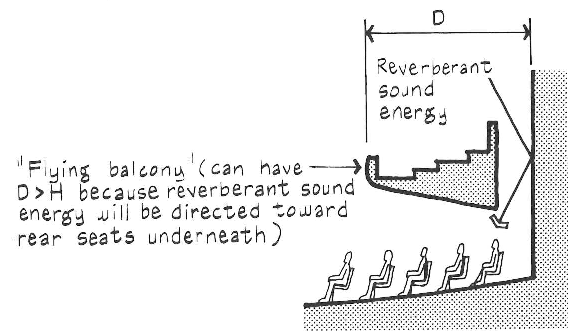
\includegraphics[keepaspectratio,scale=1]{01_att/flyingbalcony.pdf}
    \caption{\hspace{1mm}Concept of flying balcony$^2$}
    \label{fig:flyigbalcony}
\end{figure}
\\ 実際にフライングバルコニーを有するコンサートホールの例としてPhilharmonie de paris(\figref{pic_in1})が挙げられる。このホールではバルコニーがホール空間をゆるやかに二分しており、内側の空間で明瞭性を確保し、外側の空間で響きを与えている$^{\text{\cite{day2016philharmonie}}}$。
図面各種$^3$を以下に示す。
\begin{figure}[htbp]
    \centering
    \includegraphics[keepaspectratio,scale=0.2]{01_att/pic_in1.png}
    \caption{\hspace{1mm}Perspective image for interior space of Philharmonie de paris}
    \label{fig:pic_in1}
\end{figure}
\begin{figure}[htbp]
 \begin{minipage}{0.5\hsize}
  \begin{center}
   \includegraphics[scale=0.15]{01_att/PLAN_Reflector_Level.png}
  \end{center}
  \caption{\hspace{1mm}Reflector level plan}
 \end{minipage}
 \begin{minipage}{0.5\hsize}
  \begin{center}
   \includegraphics[scale=0.15]{01_att/SECTION_Long.png}
  \end{center}
  \caption{\hspace{1mm}Long cross section}
 \end{minipage}
\end{figure}
%%%%%%%%%%%%%%%%%%%%%%%%%%%%%%%%%%%%%%%%%%%%%%%%%%%%%%%%%%%%%%%%%%%%%%
\begin{figure}[htbp]
 \begin{minipage}{0.5\hsize}
  \begin{center}
   \includegraphics[scale=0.15]{01_att/PLAN_2nd_Balcony_Level.png}
  \end{center}
  \caption{\hspace{1mm}2nd balcony level plan}
 \end{minipage}
 \begin{minipage}{0.5\hsize}
  \begin{center}
   \includegraphics[scale=0.15]{01_att/SECTION_Short.png}
  \end{center}
  \caption{\hspace{1mm}Short cross section}
 \end{minipage}
\end{figure}
%%%%%%%%%%%%%%%%%%%%%%%%%%%%%%%%%%%%%%%%%%%%%%%%%%%%%%%%%%%%%%%%%%%%%%
\begin{figure}[htbp]
 \begin{minipage}{0.5\hsize}
  \begin{center}
   \includegraphics[scale=0.15]{01_att/PLAN_1st_Balcony_Level.png}
  \end{center}
  \caption{\hspace{1mm}1st balcony level plan}
 \end{minipage}
 \begin{minipage}{0.5\hsize}
  \begin{center}
   \includegraphics[scale=0.19]{01_att/suspended.png}
  \end{center}
  \caption{\hspace{1mm}Image for suspended balcony$^4$}
 \end{minipage}
\end{figure}


\addtocounter{footnote}{1}
\footnotetext{M.David Egan.ARCHITECTURAL ACOUSTICS. McGraw-Hill Book Company, p146, 1988.より引用}
\addtocounter{footnote}{1}
\footnotetext{http://www.nagata.co.jp/news/news1503.htmlより引用(2018.12.13閲覧)}
\addtocounter{footnote}{1}
\footnotetext{Márquez Cecilia. Jean Nouvel 2007 2016 : reflejos de lo contemporáneo. El Croquis Editorial, p253, 2016.より引用}

%-------------------------------------------------------------

%-------------------------------------------------------------
%-------------------------------------------------------------
\pagebreak
\section{論文構成}
本論文は、以下に示す全6章で構成される。
\\ 第1章では前節までに本研究の背景と目的、関連する既往研究の概要、本論の位置づけについて述べた。本節では、論文の構成について述べている。
\\ 第2章では、研究手法である幾何音響解析の概要、解析条件並びに解析モデルについて述べる。
\\ 第3章では、解析で得られたデータから評価をする際に用いる手法について述べる。観測点高さ間の音響物理指標値に有意な差があるかどうかを統計的な分析を行う。また、その差は人間が弁別できるほどの差であるかどうか、JND(丁度可知差異)を用いて言及する。音響物理量については理論値との比較検討を行う。
\\ 第4章では、拡散性を評価する一つの軸である音響エネルギ分布の観点から考察を行う。
\\ 第5章では、拡散性評価のもう一つの軸である反射音方向分布の観点から音場の評価を行う。
\\ 第6章では、本論の結論を述べる。